
%%******************************************************************************
%% SECTION - Materials 

%%******************************************************************************



\section{Notebooks}
\label{notebook}


\begin{table}[ht!]

	\begin{tabular}{r l|l p{12cm} }
		
		\textcolor{gray}{Especificação} &&& 	{Notebooks Dell - MODELO}\\
		\textcolor{gray}{Data} &&& 				{30/04/2014}\\
        \textcolor{gray}{Beneficiado} &&&		{DELL Computador do Brasil LTD} \\
        \textcolor{gray}{CNPJ} &&& 				{72.381.189/0006-25} \\
        \textcolor{gray}{Número Nota} &&& 		{4416982} \\
		\textcolor{gray}{Quantidade} &&& 		{3} \\
		\textcolor{gray}{Valor} &&& 			{R\$9.087,83} \\
		\textcolor{gray}{Data Sheet} &&& 		{-} \\

		\textcolor{gray}{Função no projeto} &&& {O robô ROSA terá suas funções testados no canteiro de obras da Usina Hidroelétrica Jirau. Logo, para a execução dos testes será necessário Laptops para acompanhar os mesmos e realizar as correções necessárias.  } \\
		\textcolor{gray}{Razão da Escolha} &&& {-}\\
		\textcolor{gray}{Código de Rastreamento} &&& {59270, 58129, 59271}
	\end{tabular}
\end{table}

\newpage

\begin{figure}[h!]
 \centering
 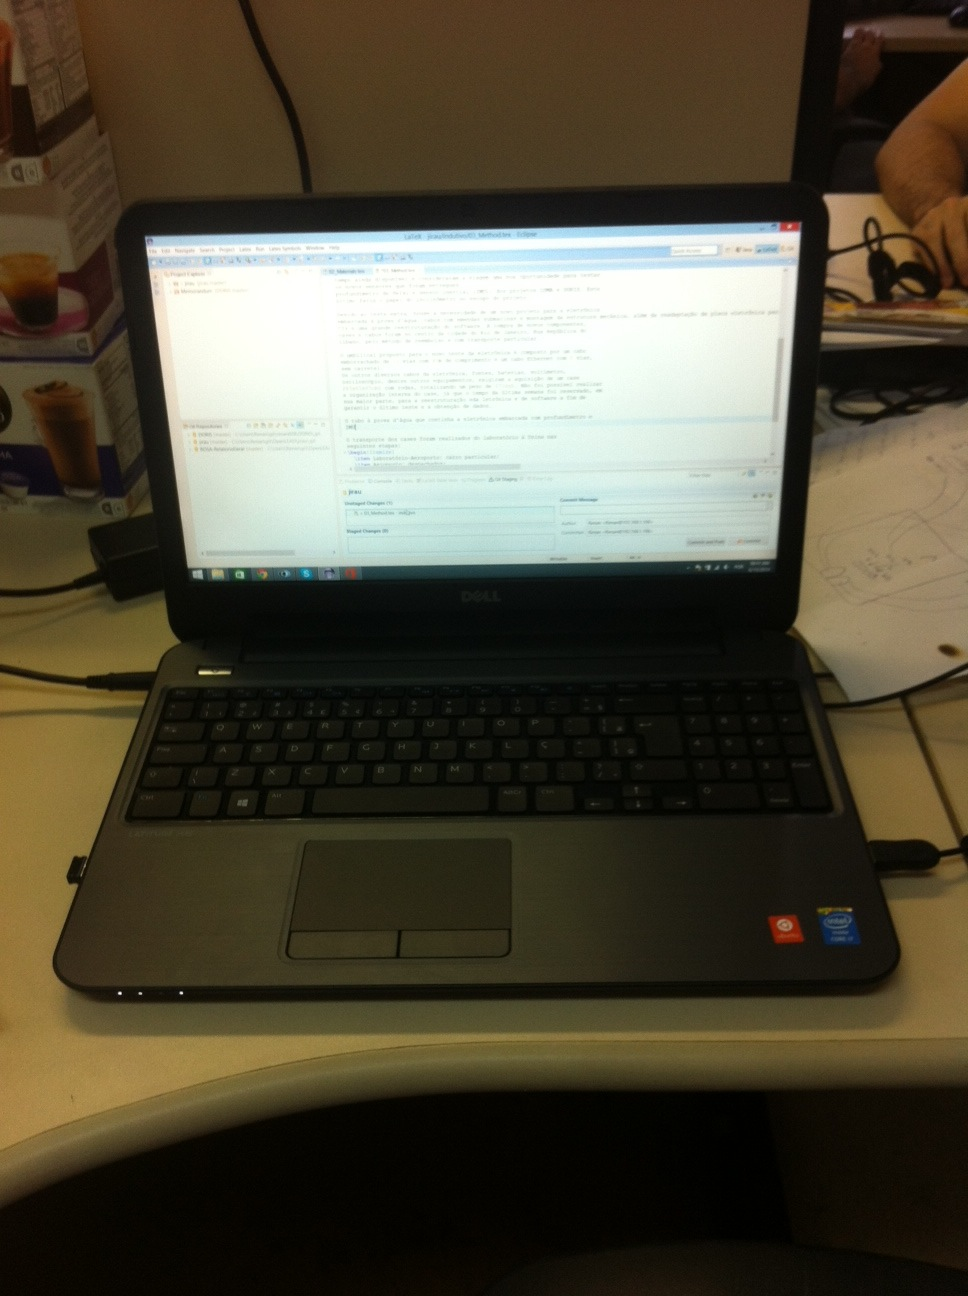
\includegraphics[width=1\columnwidth]{Notebook/foto}
 \caption{Notebook}
\end{figure}

\begin{figure}[h!]
 \centering
 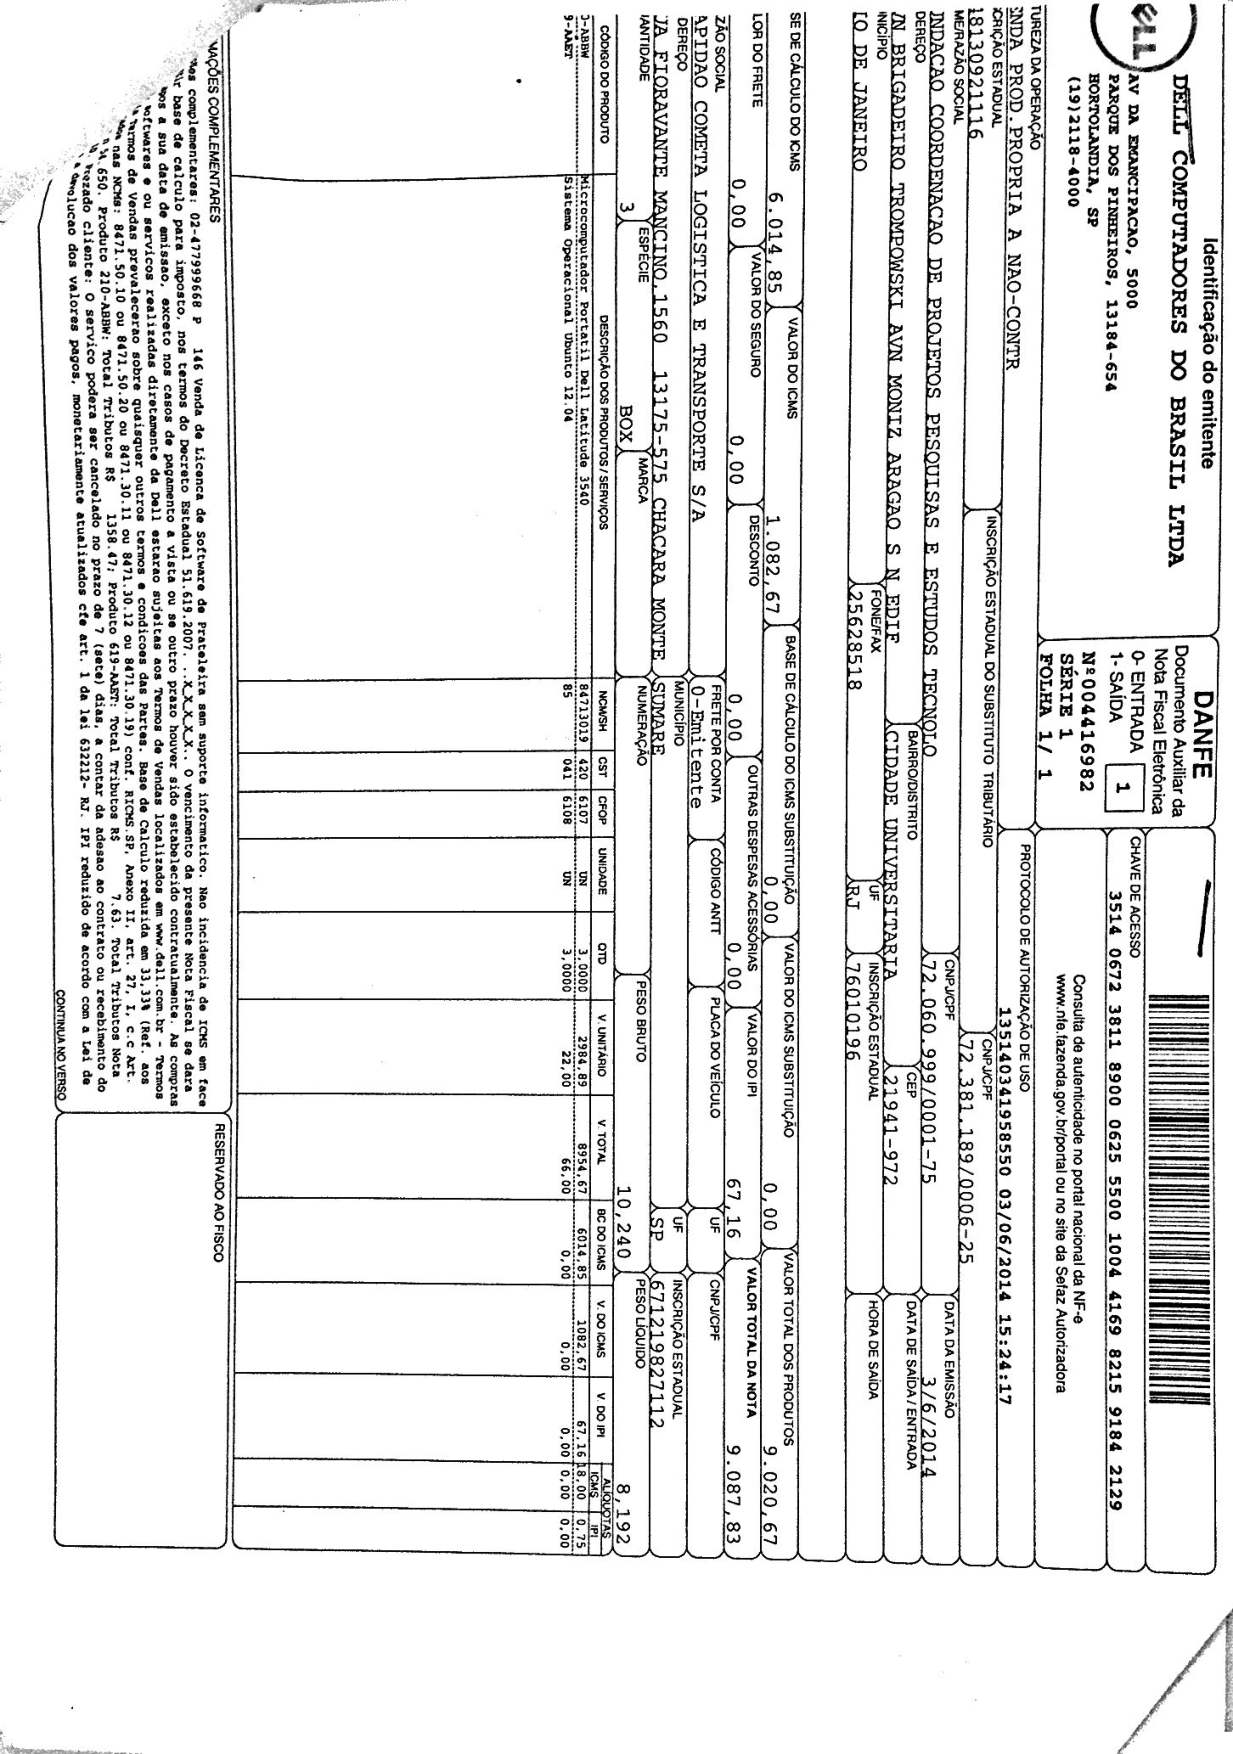
\includegraphics[width=1\columnwidth]{Notebook/nota_notebook.pdf}
 \caption{Nota Notebook}
 \end{figure}
